\section{Xilinx 7-Series Architecture}
\label{sec:7_series}
The Xilinx 7-Series devices, first introduced in 2010, follow a heterogeneous island-style architecture as discussed previously. 
Although the 7-Series was later superseded in 2013 by the UltraScale architecture, the 7-Series remains highly relevant due to its accessibility, wide availability, and compatibility with open-source tooling. 
Representative sub-families include Artix-7, Kintex-7, Virtex-7, and Zynq-7000, each designed with different performance and cost trade-offs but all follow the core 7-Series architecture.


Figure~\ref{fig:hierarchy_4} illustrates a high-level view of the hierarchical organization of a 7-Series FPGA. 
At its lowest level, the device consists of a large array of atomic components called \emph{Basic Elements of Logic}~(\textbf{BELs}). 
These BELs encompass look-up tables (\textbf{LUTs}), flip-flops (\textbf{FFs}), block RAMs (\textbf{BRAMs}), DSP slices (\textbf{DSPs}), and the configurable interconnect fabric. 
They constitute the fundamental building blocks for implementing digital circuits on the FPGA.
Note how the Tile arrangement is columnar, where each column will have only one Tile type. 

To manage this complexity, Xilinx organizes these BELs into incrementally abstract structures. 
First, \textbf{BELs} are grouped into \textbf{Sites}. 
Each Site is embedded into a \textbf{Tile}, and Tiles are further arranged into \textbf{Clock Regions}. 
In some high-density devices, multiple Clock Regions may be consolidated into one or more \textbf{Super Logic Regions}~(SLRs). 
However, for the scope of this paper, we focus on Xilinx 7-Series devices with only a single SLR.

\end{multicols}
{
    \centering
    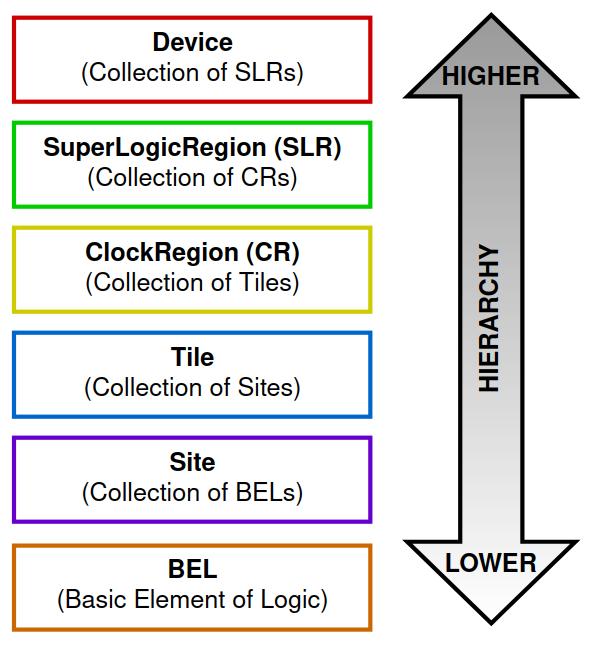
\includegraphics[valign=c, width=0.3\columnwidth]{figures/hierarchy_5.png}
    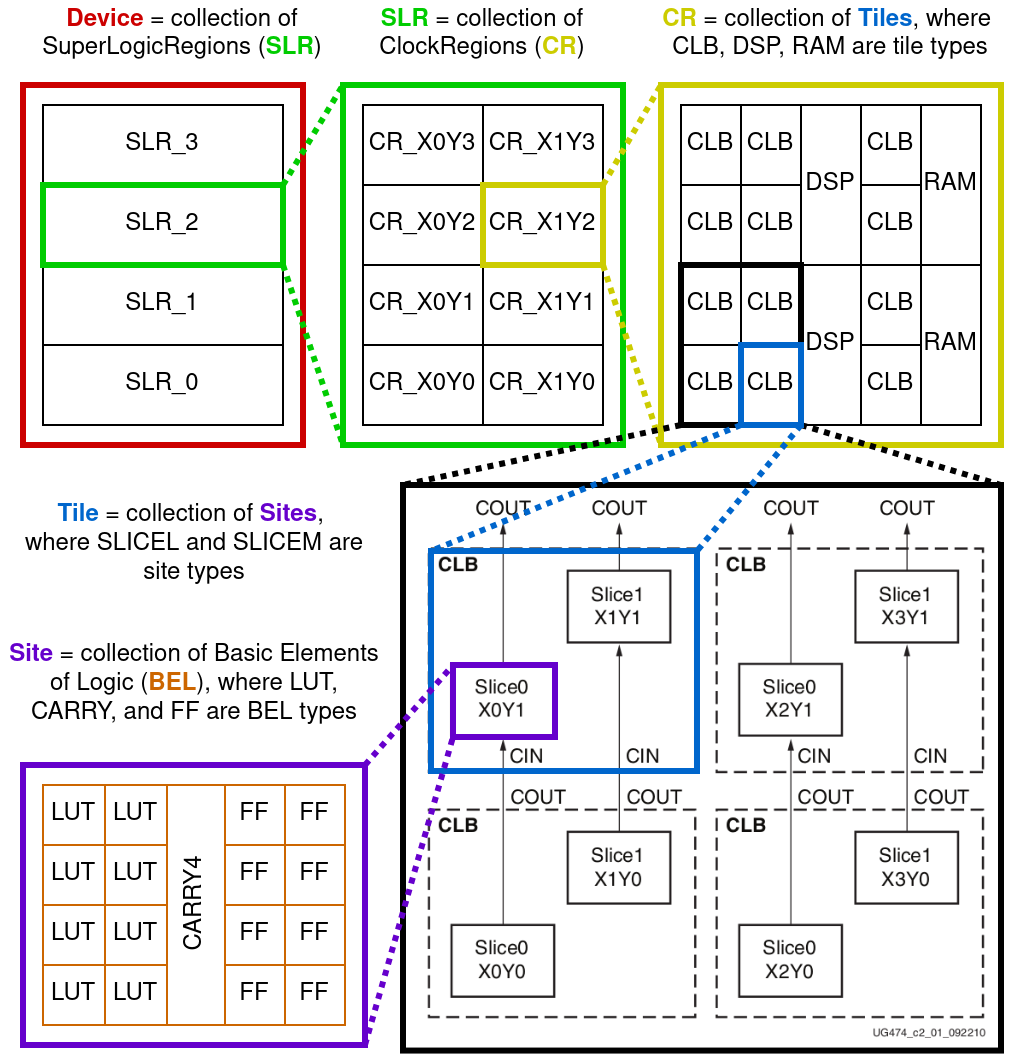
\includegraphics[valign=c, width=0.6\columnwidth]{figures/hierarchy_4.png}
    \captionof{figure}{Architecture Hierarchy of a Xilinx FPGA}
    \label{fig:hierarchy_4}
}
\vfill
\begin{multicols}{2}

\newpage
\subsection{CLB SLICEs}

In the 7-Series architecture, the term \emph{CLB} (Configurable Logic Block) refers to a \emph{CLB Tile} that contains two \emph{SLICE} Sites. 
Xilinx offers two variants of SLICE Sites: \textbf{SLICEL} and \textbf{SLICEM}.
\begin{itemize}
\item Each \texttt{SLICEL} has a set of BELs including eight \texttt{LUT}s, eight \texttt{FF}s, and one \texttt{CARRY4} adder. The \texttt{LUT} BELs in a \texttt{SLICEL} can only host \texttt{LUT} Cells. 
\item The \texttt{SLICEM} includes all the features of a \texttt{SLICEL} but its \texttt{LUT} BELs can host both \texttt{LUT} Cells, which are asynchronous ROM elements, or \texttt{RAM32M} Cells, which are synchronous 32-deep RAM elements. These cells are also referred to as \emph{Distributed RAM} in the Xilinx documentation.
    These cells can offer an alternative to the larger, more dedicated 18K-36K \texttt{RAMB18E1} cells when RAM resources are highly utilized. 
\end{itemize}
In a typical 7-Series device, approximately 75\% of the SLICE Sites are \texttt{SLICEL}s and 25\% are \texttt{SLICEM}s. 
A single CLB Tile can therefore host either two \texttt{SLICEL}s or one \texttt{SLICEL} and one \texttt{SLICEM}.
To simplify the problem space, however, we will only consider \texttt{SLICEL}s for general logic and use the dedicated \texttt{RAMB18E1} cells to implement RAM elements. 

The BELs in these SLICEs facilitate the bulk of the general programmability of the FPGA fabric. 
We will explain in detail the function and motivation behind these BELs. 


\textbf{LUTs} \quad
Combinational logic is universal to all HDL designs. 
As the their name suggests, a Look‑Up Table (LUT) map an input value to an output value. 
LUTs facilitate combinational logic by acting as tiny asynchronously‑accessed ROMs whose contents are fixed when the FPGA is programmed.  
For any boolean function, the synthesizer precalculates the boolean output to every possible input combination and stores the resulting truth table into a LUT's static memory. 
The inputs are then essentially treated as an address space that maps to a data value space in an asynchronous ROM. 
No explicit logic gates like NAND or XNOR are synthesized, contrary to what newcomers might expect from a "Field Programmable Gate Array". 

{
    \centering
    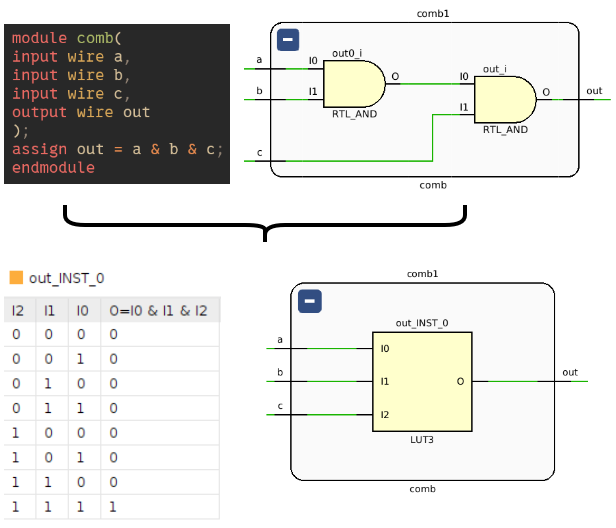
\includegraphics[width=\columnwidth]{figures/lut_synthesis.png}
    \captionof{figure}{LUT synthesis from user design}
    \label{fig:lut_synthesis}
}
\vspace{1.0cm}

In the 7‑Series devices, one LUT can facilitate any 6-input boolean function, or two 5-input functions, as long as they share the same input signals.  
The LUT can also host two independent boolean functions of up to 3 inputs each, even when the inputs are not shared.  
Functions requiring more than six unique inputs are decomposed across multiple cascaded LUTs.
Figure \ref{fig:lut_synthesis} shows an example of where a LUT is typically synthesized in a design entry. 


\textbf{FFs} \quad
FFs are synthesized to facilitate synchronous event-driven signal assignment. 
For most Verilog users, this generally means signal assignments wrapped in \texttt{always @(posedge clk)} statements. 
Figure \ref{fig:ff_synthesis} shows an example of where a FF is typically synthesized. 
The cell primitive \textbf{FDRE} is a type of FF and belongs to a family of D Flip Flops (DFFs) with Clock Enable (\texttt{CE}). 
\begin{itemize}
\item \texttt{FDCE} - DFF with CE and Asynchronous Clear
\item \texttt{FDPE} - DFF with CE and Asynchronous Preset
\item \texttt{FDSE} - DFF with CE and Synchronous Set
\item \texttt{FDRE} - DFF with CE and Synchronous Reset
\end{itemize}
In a typical HDL design, the vast majority of FFs will be synthesized as FDREs with the occasional FDSE, as it is generally good practice to keep FPGA designs synchronous. 
A FF BEL may also host a LATCH Cell, however, since they are generally bad practice in FPGA design, we will not consider latches in this paper. 

{
    \centering
    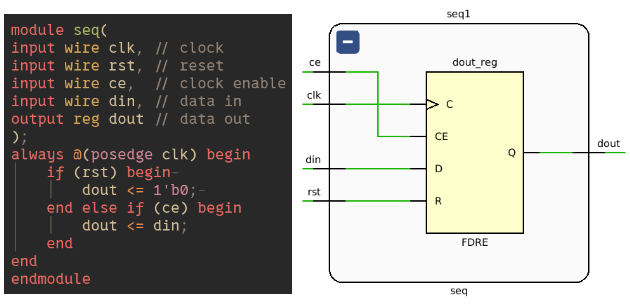
\includegraphics[width=\columnwidth]{figures/ff_synthesis.png}
    \captionof{figure}{FF synthesis from user design}
    \label{fig:ff_synthesis}
}
\vspace{1.0cm}

Up to eight (8) FFs can be placed within the same SLICE, but only if they all share a common Clock-Enable (CE) net and a common Set-Reset (SR) net.
This is because the SLICE has only one CE pin and one SR pin to interface with general routing. 
The CE and SR signals from these pins are broadcast intra-Site to all FFs within. 


\newpage
\textbf{LUT-FF Pairs} \quad
FPGA designs are very often modelled as a collection of Finite State Machines (FSM) like shown in Figure \ref{fig:fsm}.
Many times a design will also use pipelining, either to model signal buffers or shift registers, or to split up large combinational logic blocks into time slices to meet timing constraints. 
These common design structures result in many consecutive sections of combinational logic feeding into a vector of registers. 
The synthesizer naturally synthesizes these structures as consecutive pairs of LUTs feeding into FFs as shown in Figure \ref{fig:pipelining}. 
Figure \ref{fig:lut_ff_pair} shows an example of a synthesized LUT-FF Pair. 

Shown in Figure \ref{fig:intersite_intrasite} are two possible placements for a LUT-FF Pair on the physical device. 
On the right, the cells are placed across different Sites, thus the only way to route the net between the cells is through general inter-site routing. 
On the bottom left, the cells are placed within the same Site in the same lane, taking advantage of the intra-site routing without burdening the general router with additional inter-site routing. 
This is an important consideration to make while minimizing wirelength during placement. 


\vspace{1.0cm}
{
    \centering
    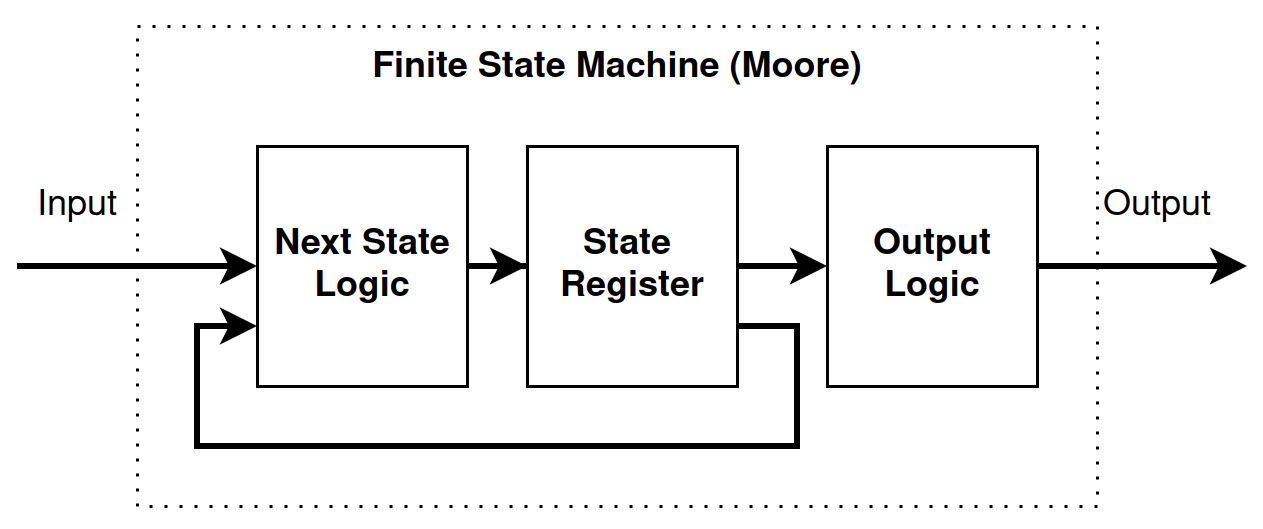
\includegraphics[width=\columnwidth]{figures/fsm.png}
    \captionof{figure}{Finite state machine (Moore)}
    \label{fig:fsm}
}
\vspace{1.0cm}

{
    \centering
    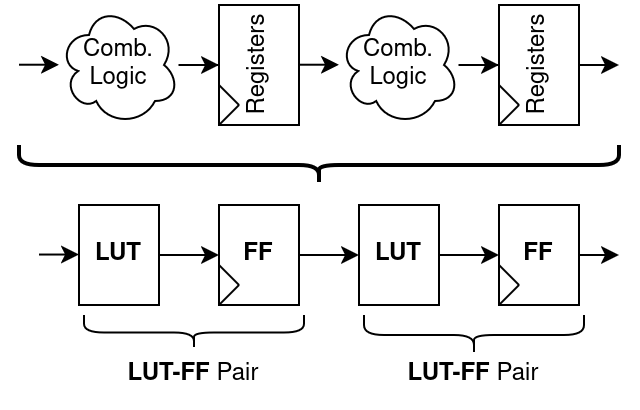
\includegraphics[width=0.9\columnwidth]{figures/pipelining.png}
    \captionof{figure}{Pipelining synthesized as consecutive LUT-FF pairs}
    \label{fig:pipelining}
}

\vfill
.
\newcolumn

{
    \centering
    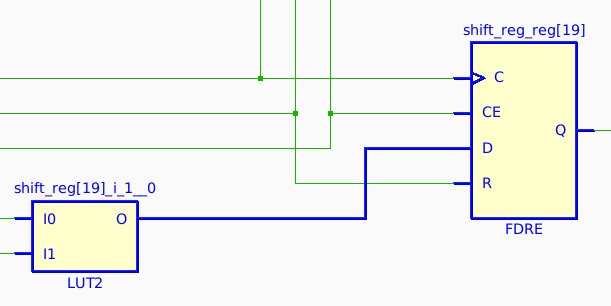
\includegraphics[width=0.9\columnwidth]{figures/lut_ff_pair.png}
    \captionof{figure}{A synthesized LUT-FF Pair}
    \label{fig:lut_ff_pair}
}
\vspace{1.0cm}

{
    \centering
    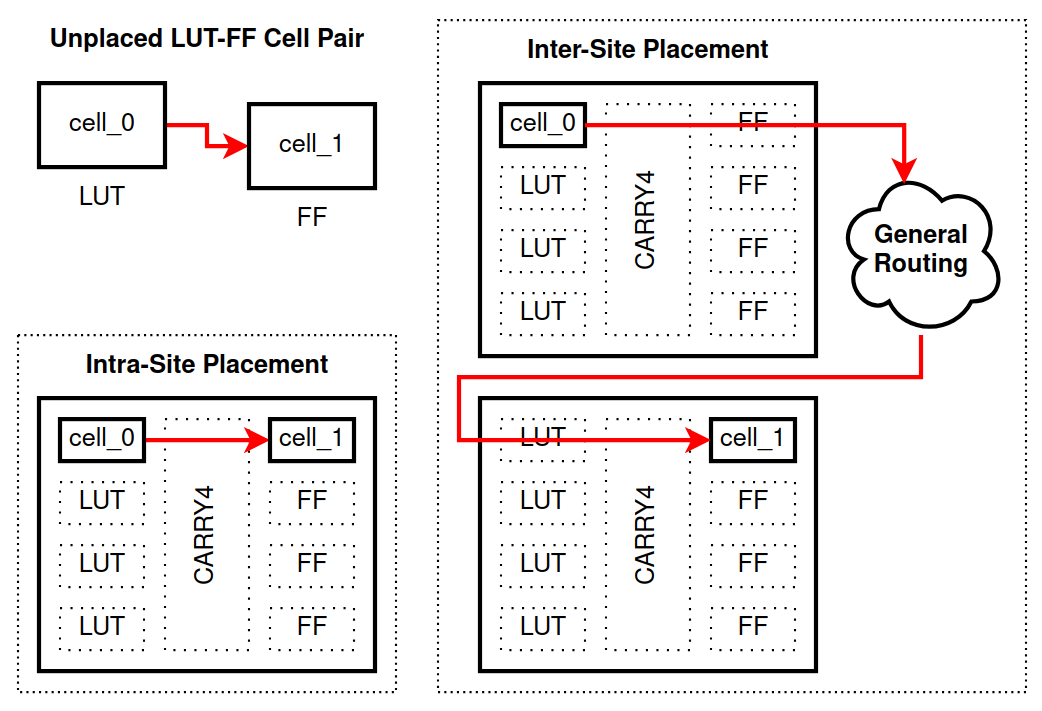
\includegraphics[width=\columnwidth]{figures/intersite_intrasite_2.png}
    \captionof{figure}{Intrasite vs Intersite LUT-FF Placement}
    \label{fig:intersite_intrasite}
}


\newpage
\textbf{CARRY} \quad
An FPGA design will also typically implement many adders, counters, subtractors, or comparators, all of which are based on binary addition. 
They are so ubiquitous that every that in the 7-Series architecture, every SLICE features a \texttt{CARRY4} BEL -- a 4-bit carry-lookahead (CLA) adder, a much better alternative to synthesizing adders via LUTs. 

\textbf{CARRY Chains} \quad
These \texttt{CARRY4} blocks can be chained across SLICEs to implement wide adders efficiently. 
The \texttt{CARRY4} BELs \emph{must} be chained vertically consecutively across SLICEs as the Carry-In (\texttt{CI}) and Carry-Out (\texttt{CO}) pins can only be routed this way. 
A \texttt{CARRY4} cell may also directly connect to LUTs and FFs, and should be placed in the same Site whenever possible to minimize wirelength. 
Shown in figure \ref{fig:carry_cell_group} shows how a \texttt{CARRY4} chain and associated LUTs and FFs can be placed across SLICEs. 


{
    \centering
    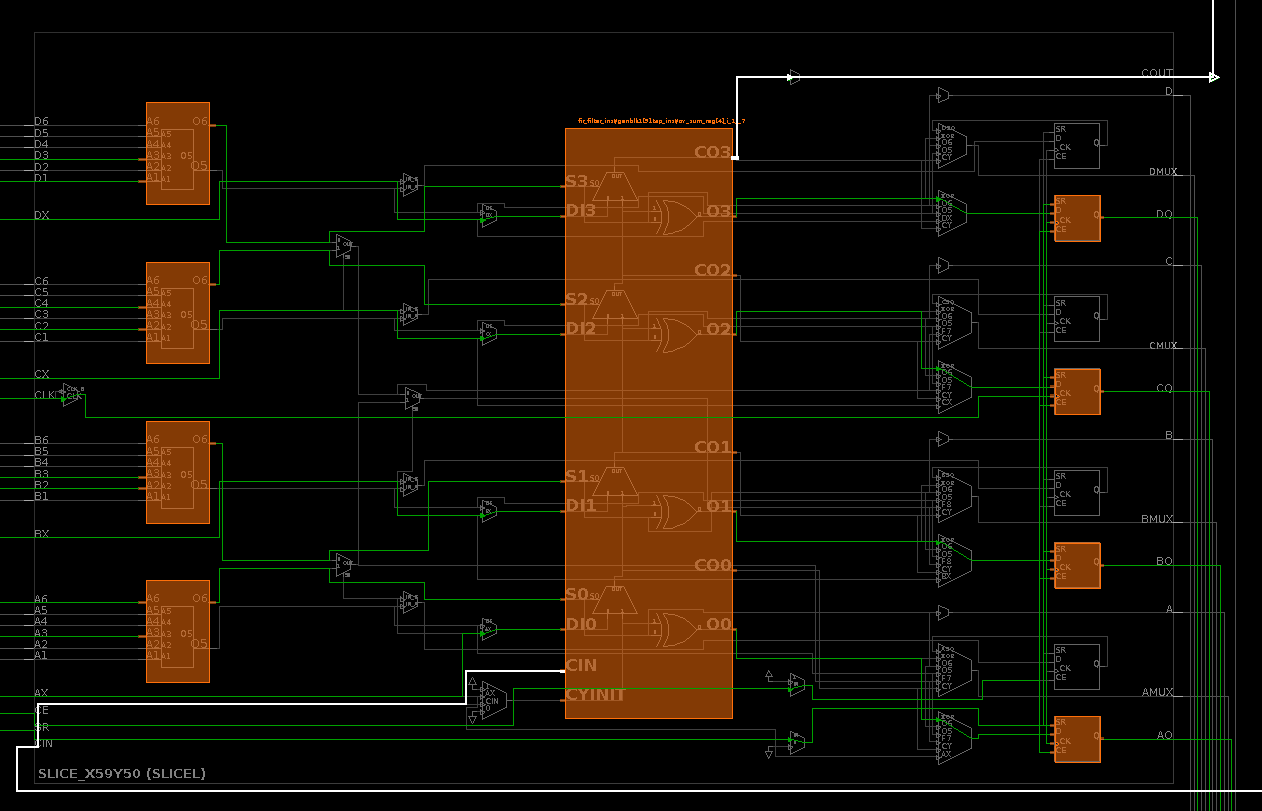
\includegraphics[width=\columnwidth]{figures/carry_cell_group.png}
    \captionof{figure}{A \texttt{SLICEL} with a \texttt{CARRY4} cell, 4 LUT cells, and 4 FF cells placed inside as shown in the Vivado device viewer}
    \label{fig:carry_cell_group}
}

{
    \centering
    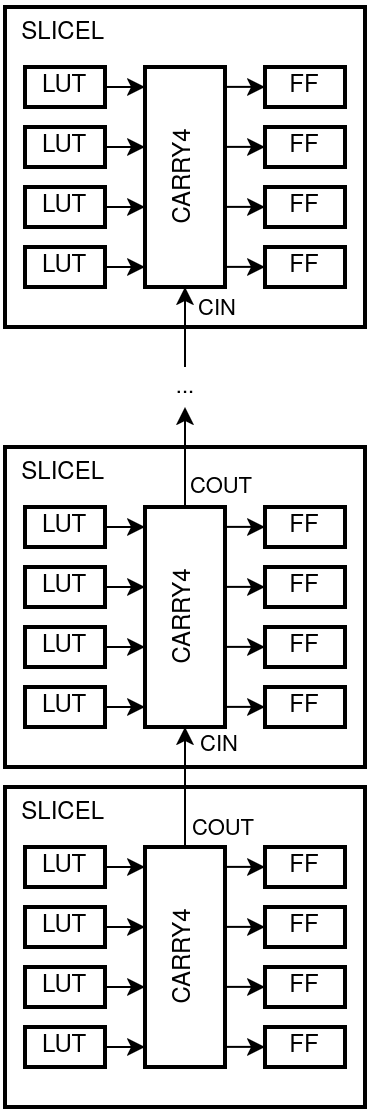
\includegraphics[valign=c, width=4.0cm]{figures/carry_chain_placement.png}
    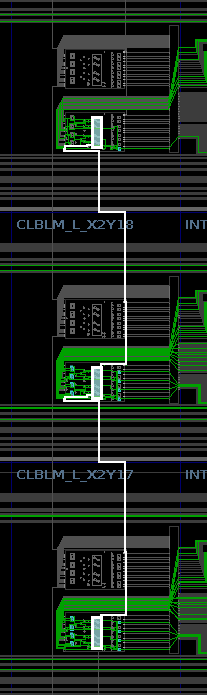
\includegraphics[valign=c, width=4.0cm]{figures/carry_chain_routes_3.png}
    \captionof{figure}{
        A \texttt{CARRY4} chain of size 3 placed across 3 SLICEs.
        \textbf{Left:} Simplified view, \textbf{Right:} As shown in the Vivado device viewer.
    }
    \label{fig:carry_cell_group}
}

\end{multicols}
% \vfill
{
    \centering
    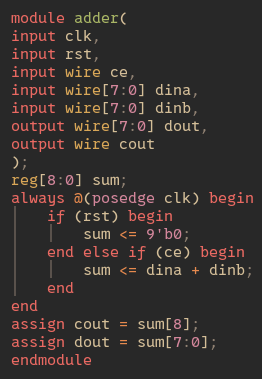
\includegraphics[valign=c, width=3.0cm]{figures/adder_synthesis.png}
    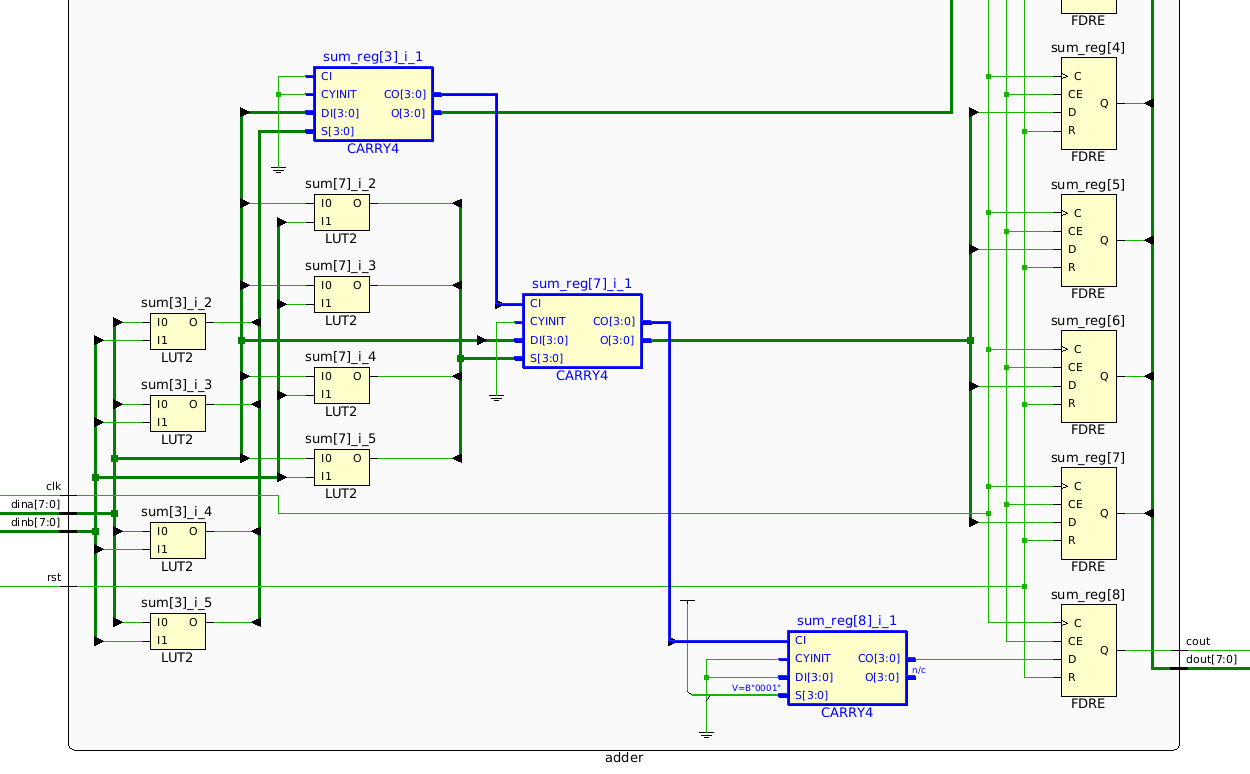
\includegraphics[valign=c, width=14.0cm]{figures/carry_chain_edif_3.png}
    \captionof{figure}{A \texttt{CARRY4} chain of size 3 as shown in the Vivado netlist viewer}
    \label{fig:carry_chain_edif}
}
\begin{multicols}{2}
\vspace{1.0cm}
.

\newpage
\subsection{DSP Slices}

\textbf{DSPs} \quad 
FPGAs are often used as low latency Digital Signal Processing (DSP) accelerators. 
Common DSP subsystems like Finite Impulse Response (FIR) filters, Fast Fourier Transform (FFTs), and convolutional neural nets (CNNs) demand fast large scale multiply-accumulate (MAC) capabilities. 
The 7-Series arhictecture integrates DSP BELs into the logic fabric called DSP48E1 that can facilitate MAC efficiently. 
The architecture hierarchy for DSPs is simple compared to CLBs and SLICEs. 
A \texttt{DSP48E1} Tile contains two \texttt{DSP48E1} Sites, each containing one \texttt{DSP48E1} BEL, which can host a \texttt{DSP48E1} Cell. 

{
    \centering
    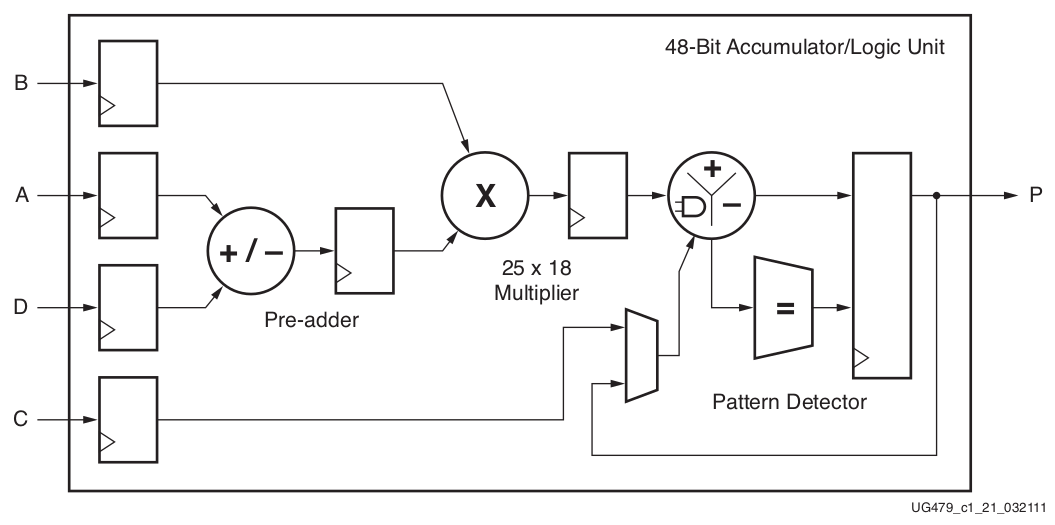
\includegraphics[width=\columnwidth]{figures/dsp_diagram.png}
    \captionof{figure}{
        Basic \texttt{DSP48E1} Slice Functionality
    }
    \label{dsp_diagram}
}
\vspace{0.5cm}

\textbf{DSP Cascades} \quad 
Wider DSP functions are supported by cascading \texttt{DSP48E1} slices in a \texttt{DSP48E1} column.
Much like \texttt{CARRY4} chains, \texttt{DSP48E1} cascades must necessarily be placed vertically consecutively across \texttt{DSP48E1} Sites. 
They are connected by three busses: \texttt{ACOUT} to \texttt{ACIN}, \texttt{BCOUT} to \texttt{BCIN}, \texttt{PCOUT} to \texttt{PCIN}.
These signal busses run directly between the vertical \texttt{DSP48E1} slices without burdening the general routing resources. 
The ability to cascade this way provides a high-performance and low-power implementation of digital signal processing systems. 

\vspace{1.0cm}
{
    \centering
    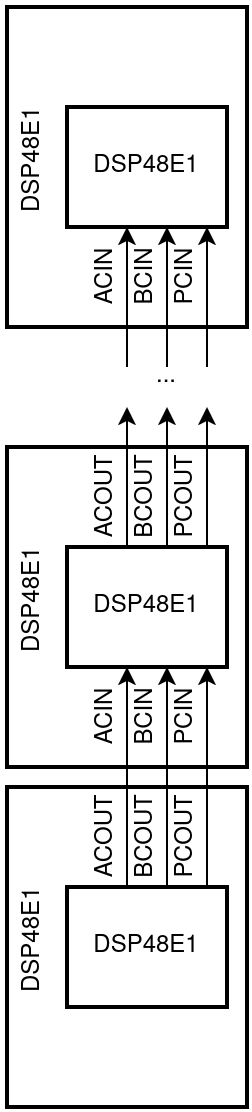
\includegraphics[valign=c, width=2.5cm]{figures/dsp_cascade_placement.png}
    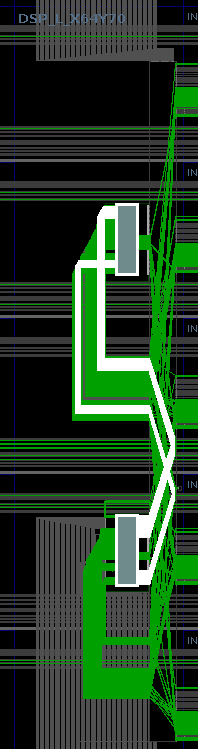
\includegraphics[valign=c, width=3.0cm]{figures/dsp_cascade_routed.png}
    \captionof{figure}{
        A \texttt{DSP48E1} cascade of size 2 placed across 2 \texttt{DSP48E1} Sites.
        \textbf{Left:} Simplified view, \textbf{Right:} As shown in the Vivado device viewer.
    }
}

\end{multicols}
{
    \centering
    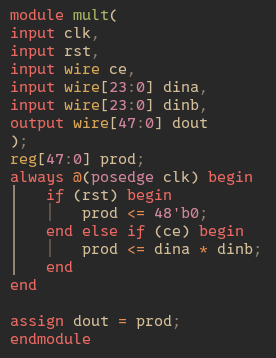
\includegraphics[valign=c, width=4.0cm]{figures/mult_synthesis.png}
    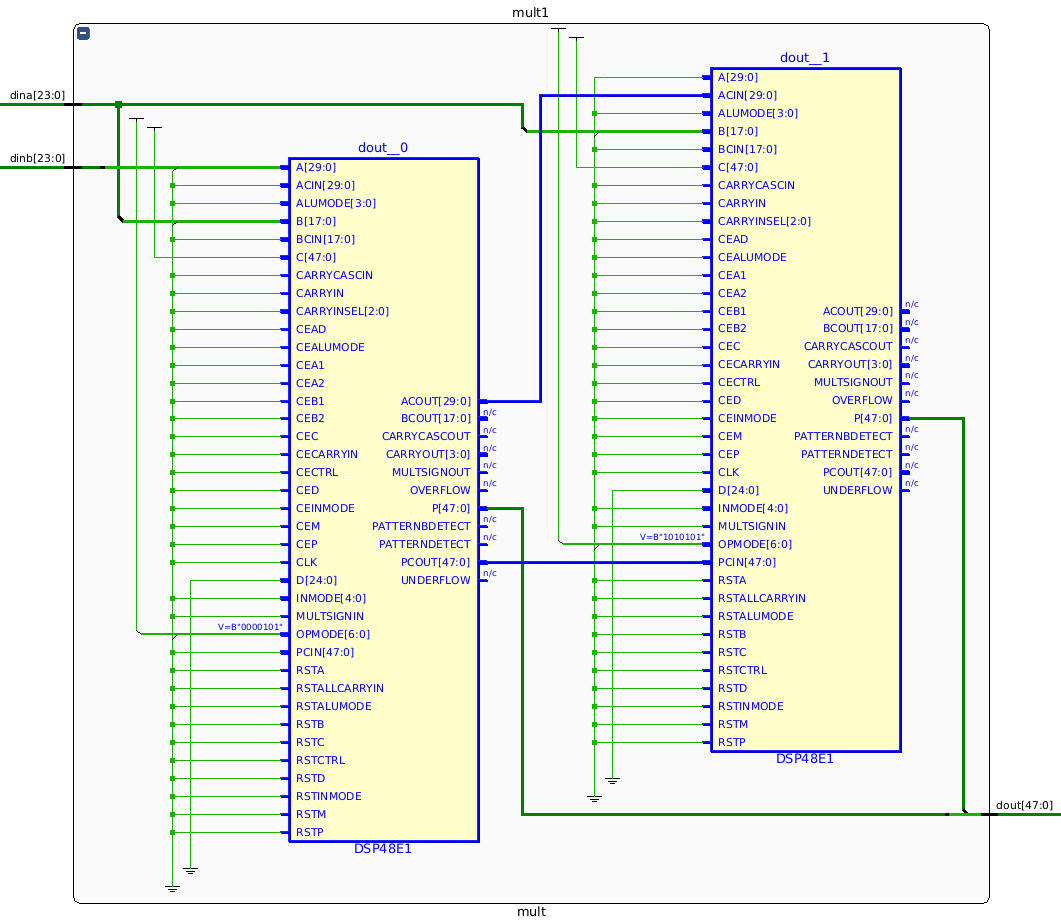
\includegraphics[valign=c, width=13.0cm]{figures/dsp_synthesis.png}
    \captionof{figure}{
        Simple multiplier synthesis from user design.
    }
    \label{mult_synthesis}
}
\begin{multicols}{2}


\newpage

\subsection{Block RAM}
In addition to SLICEs and DSPs, the 7-Series also offers dedicated Block Random Access Memory (BRAM) BELs. 
These BRAMs come in two variants: \textbf{RAMB18E1} and \textbf{RAMB36E1}. 
\begin{itemize}
\item \texttt{RAMB18E1} - 
Has a capacity of 18 Kilobits. 
It can be configured as single port RAM with dimensions ranging between (1-bit wide by 16K deep) to (18-bit wide by 1024 deep). 
It can also be configured as a (36-bit wide by 512 deep) true simple dual port RAM. 
\item \texttt{RAMB36E1} - 
Has a capacity of 36 Kilobits. 
It can be configured as single port RAM with dimensions ranging between (1-bit wide by 32K deep) to (36-bit wide by 1024 deep). 
It can also be configured as a (72-bit wide by 512 deep) simple dual port RAM. 
\end{itemize}

One BRAM Tile contains one \texttt{RAMB36E1} Site and two \texttt{RAMB18E1} Sites. 
The \texttt{RAMB36E1} Site contains one \texttt{RAMB36E1} BEL, which can host one \texttt{RAMB36E1} Cell. 
Likewise, the \texttt{RAMB18E1} Site contains one \texttt{RAMB18E1} BEL, which can host one \texttt{RAMB18E1} Cell. 

Like DSP cascades, BRAMs may also be cascaded together in a column to implement large memories efficiently, with some intermediate signals between them routed intra-Tile without burdening the general routing. 
However, unlike DSPs, large memories decomposed amongst multiple BRAMs can also be routed together through general routing. 
Furthermore, in most design scenarios, large memories will not utilize the intra-Tile signals. 

To simplify the problem space, we will not constrain large BRAMs to be cascaded together in consecutive vertical Tiles. 
We can essentially treat \texttt{RAMB18E1} and \texttt{RAMB36E1} Cells as loose, minimally constrained single cells, in contrast to the highly constrained \texttt{DSP48E1} cascades and \texttt{CARRY4} chains.

{
    \centering
    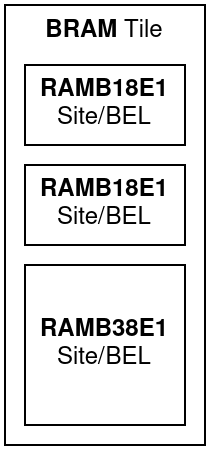
\includegraphics[valign=c, width=3.0cm]{figures/bram.png}
    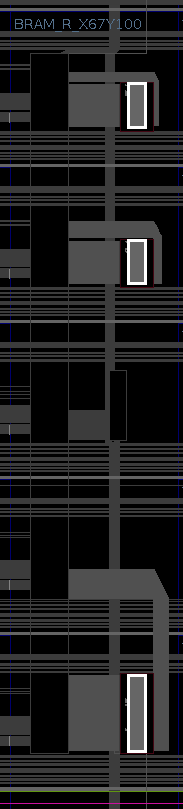
\includegraphics[valign=c, width=2.0cm]{figures/bram_tile.png}
    \captionof{figure}{
        A BRAM Tile containing two \texttt{RAMB18E1} Sites and one \texttt{RAMB36E1} Site.
        \textbf{Left:} simplified view. \textbf{Right:} as seen in the device viewer, BELs highlighted in white. 
    }
    \label{fig:bram_tile}
}

{
    \centering
    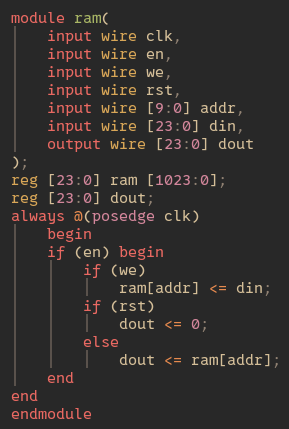
\includegraphics[valign=c, width=4.0cm]{figures/bram_synthesis.png}
    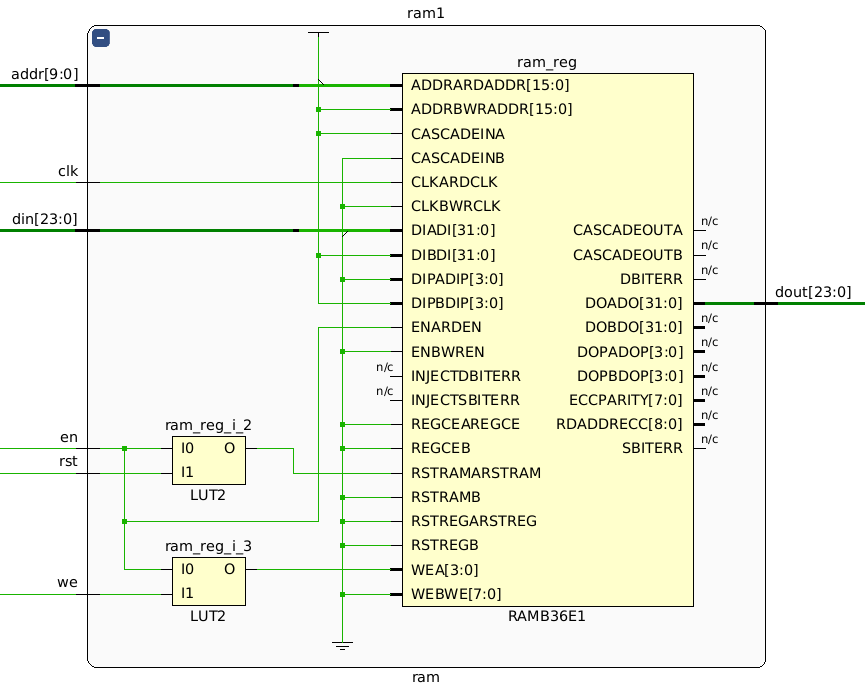
\includegraphics[valign=c, width=\columnwidth]{figures/bram_edif.png}
    \captionof{figure}{
        An example of BRAM synthesis (via inference)
    }
    \label{fig:bram_synthesis}
}

\subsection{Further Documentation}

For more in-depth details about 7-Series FPGAs, refer to the official Xilinx user guides such as:
\begin{itemize}
\item \emph{7 Series FPGAs Overview} (UG476)
\item \emph{7 Series FPGA Configurable Logic Block} (UG474)
\item \emph{7 Series Memory Resources} (UG473)
\item \emph{7 Series DSP48E1 Slice} (UG479)
\end{itemize}

This architectural context provides the necessary background for understanding how a placement algorithm should account for resource constraints and optimize performance in modern FPGA designs.


